%!TeX root = main.tex

\begin{frame}{\insertsection}{}
	\begin{itemize}
		\item Working Online
		\begin{itemize}
			\item Overleaf
			\begin{itemize}
				\item University of Melbourne, has a campus subscription to Overleaf
			\end{itemize}
				\item \LaTeX\ Base
				\item Papeeria
		\end{itemize}
		\item Working Offline
		\begin{itemize}
			\item \LaTeX\ Distributions
			\begin{itemize}
				\item MiKTex
				\item Tex Live
			\end{itemize}
			\item Third-part Editors
			\begin{itemize}
				\item TeX Studio
				\item TeX Maker
				\item Visual Studio Code
				\item Notepad
			\end{itemize}
		\end{itemize}
	\end{itemize}
\end{frame}

\begin{frame}{\insertsection}{Your First Document}
	\begin{block}{Hello World.tex}
		\inputminted[numbers=none]{latex}{./Example_Codes/FirstDoc.tex}
	\end{block}
\end{frame}

\begin{frame}{\insertsection}{Customization}
	\begin{block}{Custom Margins and Paper size}
		\inputminted[numbers=none]{latex}{./Example_Codes/SecDoc.tex}
	\end{block}
\end{frame}

\begin{frame}{\insertsection}{Text Emphasis}
	\begin{block}{Bold}
		{\mintinline{latex}{\textbf{text}}}
	\end{block}
	\begin{block}{Italics}
		{\mintinline{latex}{\textit{text}}}
	\end{block}
	\begin{block}{Underlined}
		{\mintinline{latex}{\underline{text}}}
	\end{block}
\end{frame}

\begin{frame}{\insertsection}{Images}
	\begin{block}{Images Style 1}
	\inputminted[numbers=none]{latex}{./Example_Codes/images1.tex}
	\end{block}
\end{frame}

\begin{frame}{\insertsection}{Images}
	\begin{block}{Images Style 2}
		\inputminted[numbers=none]{latex}{./Example_Codes/images2.tex}
	\end{block}
\end{frame}

\begin{frame}{\insertsection}{Math typing and the \mintinline{latex}{amsmath} package}
	\mintinline{latex}{\usepackage{amsmath}}
	\begin{block}{Numbered environments}
		\mintinline{latex}{eqaution}, \mintinline{latex}{gather}, \mintinline{latex}{align}
	\end{block}
	\begin{block}{Unnumbered environments}
		\mintinline{latex}{eqaution*}, \mintinline{latex}{gather*}, \mintinline{latex}{align*}
	\end{block}
	\begin{block}{Inline}
		\mintinline{latex}{$y = mx + c$}
	\end{block}
\end{frame}

\begin{frame}{\insertsection}{Sectioning}
	\mintinline{latex}{\tableofcontents}
	\begin{block}{Numbered}
		\mintinline{latex}{\section{Text}}, \mintinline{latex}{\subsection{Text}} ...
	\end{block}
	\begin{block}{Unnumbered}
	\mintinline{latex}{\section*{Text}}, \mintinline{latex}{\subsection*{Text}} ...
	\end{block}
\end{frame}

\begin{frame}{\insertsection}{Tables}
		\begin{block}{Example Table}
		\inputminted[numbers=none]{latex}{./Example_Codes/table.tex}
	\end{block}
\end{frame}

\begin{frame}{\insertsection}{Tables}
	\begin{figure}
		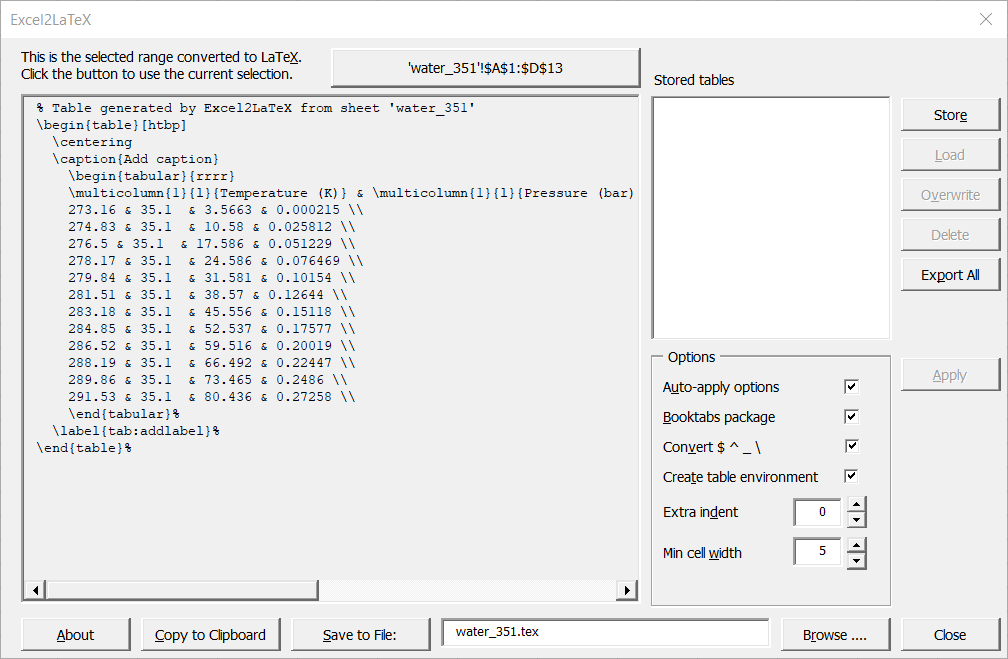
\includegraphics[width=0.4\textwidth]{./Images/excel2latex.png}
	\end{figure}
	Use Excel2LaTeX instead, it provides automatic generation of \LaTeX\ code from excel sheets.
	\blfootnote{Excel2LaTeX -- \url{https://ctan.org/pkg/excel2latex?lang=en}}
\end{frame}

\begin{frame}{Other Nice Packages}
	\begin{itemize}
		\item \mintinline{latex}{amssymb}\\
		More mathematical symbols from AMS
		\item \mintinline{latex}{pdfpages}\\
		Ability to include and splice external PDFs into your \LaTeX\ document
		\item \mintinline{latex}{siunitx}\\
		SI unit formatting and decimal alignment in tables
		\item \mintinline{latex}{csvsimple}\\
		Read .csv files to automatically create tables
		\item \mintinline{latex}{booktabs}\\
		Nicer looking table dividers
		\item \mintinline{latex}{fancyhdr}\\	
		Headers for documents	
	\end{itemize}
\end{frame}

\begin{frame}{Complimentary Programs}
	\begin{itemize}
		\item IguanaTeX\\
		\LaTeX\ in Power Points
		\item Inkscape\\
		Vector image editor
		\item Microsoft Visio\\
		Visual editor for flowcharts and diagrams\\
		My addon for \LaTeX\ in Visio (\url{https://github.com/huanga2/VSTO_LaTeX})
	\end{itemize}
\end{frame}

\begin{frame}{Further sources}
	\begin{itemize}
		\item Google
		\item TeX StackExchange
		\item Comprehensive TeX Archive Network -- \url{https://ctan.org/}
		\item Overleaf
		\item Math symbols -- \url{https://oeis.org/wiki/List_of_LaTeX_mathematical_symbols}
	\end{itemize}
\end{frame}